\documentclass{article}
\usepackage[T1,T2A]{fontenc}
\usepackage[utf8]{inputenc}
\usepackage[english,russian]{babel}
\usepackage{cmap}
\usepackage{hyperxmp}
\usepackage[colorlinks,linkcolor=blue]{hyperref}
\usepackage[landscape,left=0.1cm, right=.1cm, top=0.1cm, bottom=1cm,paperwidth=210mm,paperheight=297mm]{geometry}
\usepackage{stmaryrd}
\usepackage{tabularx}
\usepackage{enumitem}
\usepackage{fancyhdr}


\cfoot{\vspace*{-1cm}\small\ccbysa\ Vitaly Repin, 2014. This work is licensed under a \myhref{http://creativecommons.org/licenses/by-sa/4.0/}{Creative Commons Attribution-ShareAlike 4.0 International License}}
\pagestyle{fancy}

\usepackage{multicol}

\usepackage[dvipsnames]{xcolor}
\usepackage{copyrightbox}

\usepackage{tikz}
\usepackage{calc}
\usepackage{ccicons}
\usetikzlibrary{shapes.misc}
\usetikzlibrary{mindmap}

\graphicspath{{pics/}}

\newcommand{\nn}{\textbullet}

\newsavebox{\one}\newsavebox{\two}\newsavebox{\three}\newsavebox{\four}
\newlength{\onelen}\newlength{\twolen}\newlength{\threelen}\newlength{\fourlen}

\hypersetup{%
pdftitle={%
Серебряный век русской экономической мысли: П.Б. Струве, Н.К. Дмитриев, С.Н. Булгаков, М.И. Туган-Барановский, А.Д. Билимович. Конспект лекций.},
pdfauthor={Vitaly Repin},
pdfcopyright={This work is licensed under Creative Commons Attribution-ShareAlike 4.0 International License},
pdfsubject={История русской экономической мысли: П.Б. Струве, Н.К. Дмитриев, С.Н. Булгаков, М.И. Туган-Барановский, А.Д. Билимович},
pdfkeywords={Струве, Дмитриев, Булгаков, Туган-Барановский, Билимович, экономика, история, ВШЭ},
pdflicenseurl={http://creativecommons.org/licenses/by-sa/4.0/},
pdfcaptionwriter={Vitaly Repin},
pdfcontactcity={Espoo},
pdfcontactcountry={Finland},
pdfcontactemail={vitaly.repin@gmail.com},
pdflang={ru}
}

\newcommand{\myhref}[2]{\textcolor{blue}{\href{#1}{\textcolor{blue}{#2}}}}

\begin{document}

\newcommand{\elem}[2]{
\begin{tabularx}{9cm}{|lX|}
\hline
\multicolumn{2}{|c|}{\bf #1}\\
\hline
#2\\
\hline
\end{tabularx}
}

\newcommand{\setheights}{
\settoheight{\twolen}{\usebox{\two}}
\settoheight{\onelen}{\usebox{\one}}
\settoheight{\threelen}{\usebox{\three}}
}

%% Булгаков
\sbox{\two}{%
\elem{Религиозное экономическое мировоззрение}{
\nn&Прошел путь от марксизма к <<идеализму>> и религиозному экономическому мировоззрению;\\
\nn&Практический смысл п/э --- указание способов $\shortuparrow$ народного богатства, \emph{как условия духовного развития личности и общества.} <<Идеализм>> --- политика, отвечающая этому требованию;\\
\nn&Идея справедливости и эффективности: $\shortuparrow$ общественного богатства означает $\shortuparrow$ объема материальных благ при ${\neg}{\shortuparrow}$ неравенства их распределения;\\
\nn&Форма собственности оценивается по влиянию на $\shortuparrow$ общественного богатства;\\
\nn& Необходима нравственная оценка экономической жизни и экономической науки.}}


\sbox{\one}{%
\elem{Критика Маркса}{
\nn& Начало отхода от марксизма --- с попытки доказать универсальность тенденции концентрации капитала~[1]. Булгаков выяснил, что для сельского хозяйства это не так;\\
\nn& Маркс преувеличивает возможности общественной науки и недооценивает границы социального познания;\\
\nn& Опасно переносить тенденции настоящего в будущее;\\
\nn& Маркс рассматривает общественные и экономические процессы исключительно с точки зрения материальной стороны.}}

\sbox{\three}{
\elem{Отношение к маржинализму}{
\nn& Модель <<экономического человека>> -- извращение сути человека, идейный фантом;\\
\nn& Органическая целостность хозяйства: хозяйство как целое --- предпосылка отдельных хозяйственных актов, а не наоборот ($\neg$ австрийцы).}}

\setheights
\vspace*{.5cm}
\centerline{\href{http://commons.wikimedia.org/wiki/File:Sbulgakov.jpg}{\copyrightbox{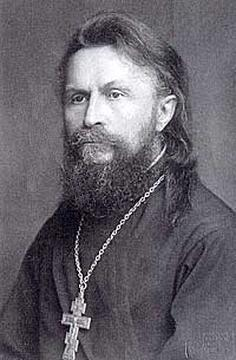
\includegraphics[height=8cm,keepaspectratio]{Sbulgakov}}{By unknown photographer in the beginning of XX century [CC0], via Wikimedia Commons}}}
\vspace*{-2cm}
\begin{center}
\begin{tikzpicture}[text width=2.7cm, align=flush center,
grow cyclic,
level 1/.style={level distance=3.5cm,sibling angle=90},
level 2/.style={text width=2cm, font=\footnotesize, level distance=3cm,sibling angle=30}]
\node[text width=3.2cm] {\textsc{\myhref{http://ru.wikipedia.org/wiki/\%D0\%91\%D1\%83\%D0\%BB\%D0\%B3\%D0\%B0\%D0\%BA\%D0\%BE\%D0\%B2\%2C_\%D0\%A1\%D0\%B5\%D1\%80\%D0\%B3\%D0\%B5\%D0\%B9_\%D0\%9D\%D0\%B8\%D0\%BA\%D0\%BE\%D0\%BB\%D0\%B0\%D0\%B5\%D0\%B2\%D0\%B8\%D1\%87}{\textbf{С.Н. Булгаков}} (1871--1944)}}
  child[sibling angle=180, level distance=4.6cm] { node[text height=\onelen, text width=9cm, anchor=east] (one) {\usebox{\one}}
  }
  child[level distance=4.6cm] { node[text height=\threelen, text width=9cm,anchor=west] {\usebox{\three}}
  }
  child[sibling angle=-90, level distance=2cm, text width=9cm, text height=\twolen, anchor=north] { node {\usebox{\two} }
};
\begin{scope}[every annotation/.style={font=\normalsize, fill=white, text width=9cm}]
\node [annotation, below] at (one.south) {
\textbf{Избранные труды}\medskip
\begin{enumerate}[label={[\arabic*]}]
\item \myhref{http://nasledie.enip.ras.ru/ras/view/publication/general.html?id=45124851}{Капитализм и земледелие}, 1900\,г.
\item Об экономическом идеале, 1903\,г.
\item \myhref{http://nasledie.enip.ras.ru/ras/view/publication/general.html?id=43419244}{От марксизма к идеализму}, 1903\, г.
\item Краткий очерк политэкономии, 1906\,г.
\item Народное хозяйство и религиозная личность, 1909\,г.
\item \myhref{http://nasledie.enip.ras.ru/ras/view/publication/general.html?id=43523569}{Философия хозяйства}, 1912\,г.
\item \myhref{http://nasledie.enip.ras.ru/ras/view/publication/general.html?id=42085803}{Христианство и социализм}, 1917\,г.
\end{enumerate}
};
\end{scope}
\end{tikzpicture}
\end{center}

\newpage
%% Туган-Барановский

\sbox{\one}{
\elem{Социализм как положительное учение [3]}{
\nn&Социализм максимизирует Функцию Общественной Полезности (ФОП) $\Rightarrow$ синтез трудовой и субъективной теорий стоимости возможен только при нем;\\
\nn&План при социализме должен учитывать как предельную полезность ($MU$), так и трудовые затраты;\\
\nn&Для определения $MU$ при социализме предлагается использовать <<механизм нащупывания>> (сравни с \myhref{http://en.wikipedia.org/wiki/Walrasian_auction}{tâtonnement Вальраса});\\
\nn&Цены могут отклоняться от пропорции с трудовыми затратами, если это в интересах общества;\\
\nn&Банковские деньги (1918 г.) --- прообраз денег при социализме (условная единица измерения цен), так как они оторваны от реальности, условны;\\
\nn&Идеи Т.-Б. про <<социализм как положительное учение>> --- в стороне от генеральной линии развития экономической мысли.
}}

\sbox{\two}{
\elem{Теория циклов и кризисов [4]}{
\nn&Теория циклов и кризисов --- вклад Т.-Б. в мировую науку, он заложил основы нового подхода к проблеме деловых циклов;\\
\nn&Кризисы происходят из-за антагонистической природы капитализма (труд/капитал). Капитал $\rightarrow$ неограниченному расширению, но нет планомерного распределения общественного производства
между предметами потребления и средствами производства;\\
\nn&Инвестиции -- наиболее важный элемент совокупного спроса (сравни с Кейнсом);\\
\nn& Внимание к динамике цен на базисные товары (уголь, железо\dots Сравни с Кондратьевым);\\
\nn&Общее перепроизводство --- из-за нарушения равновесия на одном рынке (передается на всю экономику). Кредит --- лишь катализатор процесса!\\
\nn&Периодичность кризисов: т.к. свободный денежный капитал накапливается в банках (резервуарах) и в итоге $\shortuparrow$ инвестиции в условиях невозможности регулировать пропорции производства и незнания спроса.}}

\sbox{\three}{
\elem{\mathstrut\parbox{6cm}{Синтез трудовой и субъективной\\ \centerline{теорий стоимости}}}{
\nn&Учитель экономистов, работавших в советское время (например, Н.Д. Кондратьева);\\
\nn& Попытка примирения трудовой (ТС) и субъективной (MU) теорий стоимости (т.к. человек --- в центре и там, и там);\\
\nn& <<Теорема>> Т.-Б. (для воспроизводимых благ, доказана Н.А. Столяровым): $MU_1 / MU_2 = TC_1 / TC_2.$ Выполняется в максимуме Функции Общественной Полезности (ФОП).
}}

\setheights
\vspace*{.5cm}
\centerline{\copyrightbox{\myhref{http://commons.wikimedia.org/wiki/File\%3AMikhail_Ivanovich_Tugan-Baranovskij.jpg}{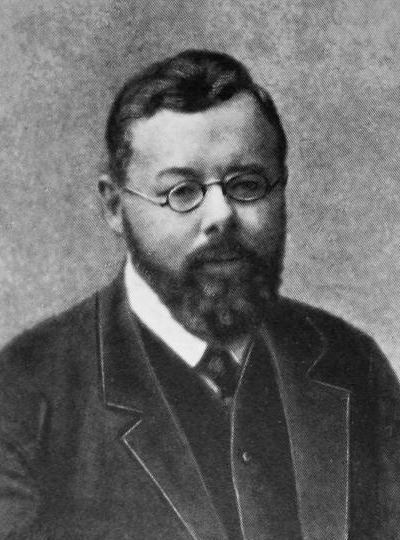
\includegraphics[height=6.2cm,keepaspectratio]{Mikhail_Ivanovich_Tugan-Baranovskij}}}{See page for author [Public domain], via Wikimedia Commons}}
\vspace*{-3.4cm}
\begin{center}
\begin{tikzpicture}[text width=2.7cm, align=flush center,
grow cyclic,
level 1/.style={level distance=3.5cm,sibling angle=90},
level 2/.style={text width=2cm, font=\footnotesize, level distance=3cm,sibling angle=30}]
\node[text width=3.2cm] {\textsc{\myhref{http://ru.wikipedia.org/wiki/\%D0\%A2\%D1\%83\%D0\%B3\%D0\%B0\%D0\%BD-\%D0\%91\%D0\%B0\%D1\%80\%D0\%B0\%D0\%BD\%D0\%BE\%D0\%B2\%D1\%81\%D0\%BA\%D0\%B8\%D0\%B9\%2C_\%D0\%9C\%D0\%B8\%D1\%85\%D0\%B0\%D0\%B8\%D0\%BB_\%D0\%98\%D0\%B2\%D0\%B0\%D0\%BD\%D0\%BE\%D0\%B2\%D0\%B8\%D1\%87}{\textbf{М.И. Туган-Барановский}} (1865--1919)}}
  child[sibling angle=180, level distance=4.6cm] { node[text height=\onelen, text width=9cm, anchor=east] (one) {\usebox{\one}}
  }
  child[level distance=4.6cm] { node[text height=\threelen, text width=9cm,anchor=west] {\usebox{\three}}
  }
  child[sibling angle=-90, level distance=2cm, text width=9cm, text height=\twolen, anchor=north] { node {\usebox{\two} }
};
\begin{scope}[every annotation/.style={font=\normalsize, fill=white, text width=9cm}]
\node [annotation, below] at (one.south) {
\textbf{Избранные труды}\medskip
\begin{enumerate}[label={[\arabic*]}]
\item Учение о предельной полезности, 1890\,г.
\item Основы политэкономии, 1909\,г.
\item \myhref{http://nasledie.enip.ras.ru/ras/view/publication/general.html?id=47003536}{Социализм как положительное учение}, 1918\,г.
\item Периодические промышленные кризисы. История английских кризисов. Общая теория кризисов (4-е издание), 1923\, г.
\end{enumerate}
};
\end{scope}
\end{tikzpicture}
\end{center}
\newpage

%% Билимович
\sbox{\one}{
\elem{Методология}{
\nn& Каузальный подход, \emph{дополненный} статистическими исследованиями (прежде всего для оценки качества теории);\\
\nn& Проводил четкое различие между причинными и функциональными связями;\\
\nn& Эмпирические закономерности не универсальны. Часто мы не знаем при каких условиях они сохраняют свою силу;\\
\nn& Необходимость использования математики при решении теоретических проблем (сравни с В.К. Дмитриевым);\\
\nn& Методологический оппонент П.Б. Струве (каузальный подход \emph{versus} статистико-вероятностный).
}}

\sbox{\three}{
\elem{Защита дедуктивной теории цены}{
\nn& Как и П.Б. Струве, рассуждал о цене, а не о ценности;\\
\nn& Исходил из принципа оптимальности --- наилучшего использования индивидом имеющихся ресурсов для достижения своих целей;\\
\nn& Цепочка: потребность $\rightarrow$ полезность хоз. благ $\rightarrow$ субъективная ценность $\rightarrow$ цена;\\
\nn& Понятие \emph{коллективной} потребности (группа, а не только индивид);\\
\nn& Применение принципа редкости к труду: трудовые возможности ограничены, как и все остальные блага $\Rightarrow$ интересуемся затратами труда;\\
\nn& У дедуктивной статической равновесной теории есть потенциал к исследованию динамических проблем, процессов.
}}

\sbox{\two}{
\elem{Жизнь и судьба}{
\nn&С 1920 г. --- в эмиграции, с 1948 г. --- в Беркли;\\
\nn&Непримиримый противник марксизма.
}}

\setheights
\begin{center}
\begin{tikzpicture}[text width=2.7cm, align=flush center,
grow cyclic,
level 1/.style={level distance=3.5cm,sibling angle=90},
level 2/.style={text width=2cm, font=\footnotesize, level distance=3cm,sibling angle=30}]
\node[text width=3.2cm] {\textsc{\myhref{http://ru.wikipedia.org/wiki/\%D0\%91\%D0\%B8\%D0\%BB\%D0\%B8\%D0\%BC\%D0\%BE\%D0\%B2\%D0\%B8\%D1\%87\%2C_\%D0\%90\%D0\%BB\%D0\%B5\%D0\%BA\%D1\%81\%D0\%B0\%D0\%BD\%D0\%B4\%D1\%80_\%D0\%94\%D0\%BC\%D0\%B8\%D1\%82\%D1\%80\%D0\%B8\%D0\%B5\%D0\%B2\%D0\%B8\%D1\%87}{\textbf{А.Д. Билимович}} (1876--1963)}}
  child[sibling angle=180, level distance=4.6cm] { node[text height=\onelen, text width=9cm, anchor=east] {\usebox{\one}}
  }
  child[level distance=4.6cm] { node[text height=\threelen, text width=9cm,anchor=west] {\usebox{\three}}
  }
  child[sibling angle=90, level distance=3.5cm, text width=9cm, text height=\twolen, anchor=north] { node {\usebox{\two} }
};
\end{tikzpicture}
\end{center}

%% Дмитриев
\sbox{\three}{
\elem{Основные результаты}{
\nn&Демонстрация возможностей математики в экономической науке;\\
\nn&Модель полных затрат: представил издержки через количество труда, прямо или косвенно использованного для производства (а не цены!), чем избавил теорию цен от логического круга;\\
\nn&Определил прибыль и цены всех товаров в зависимости от условий производства товаров, потребляемых работниками, и уровня заработной платы;\\
\nn&<<Самовоспроизводящийся капитал>>: для модели Дмитриева необязателен живой труд, его можно заменить трудом машины, способной к самовоспроизводству;\\
\nn&Связь процесса определения рыночных цен с проблемами конкуренции: \emph{свободная конкуренция} не снижает цену до издержек, а \emph{<<подтягивает>> издержки к цене} ($\neg$ Рикардо);\\
\nn&<<Почти строго>> дедуктивная система рассуждений: при обсуждении проблем конкуренции обращается к эмпирическим данным;\\
\nn&Не только цена товаров с горизонтальной кривой издержек (КИ), \emph{но и цена товаров с $\shortuparrow$ КИ} определяется через ограничение со стороны спроса. Спрос же зависит от предпочтений индивидов (связь с теорией предельной полезности).
}}

\sbox{\one}{
\elem{Научные интересы}{
\nn&Первый русский экономист-математик;\\
\nn&Развитие теории ценностей Рикардо;\\
\nn&Развитие теории конкуренции и монополии;\\
\nn&Соединение теории издержек с теорией предельной полезности;\\
\nn&Анализ функции спроса.
}}


\setheights
\begin{center}
\begin{tikzpicture}[text width=2.7cm, align=flush center,
grow cyclic,
level 1/.style={level distance=3.5cm,sibling angle=90},
level 2/.style={text width=2cm, font=\footnotesize, level distance=3cm,sibling angle=30}]
\node[text width=3.2cm] (main) {\textsc{\myhref{http://ru.wikipedia.org/wiki/\%D0\%94\%D0\%BC\%D0\%B8\%D1\%82\%D1\%80\%D0\%B8\%D0\%B5\%D0\%B2\%2C_\%D0\%92\%D0\%BB\%D0\%B0\%D0\%B4\%D0\%B8\%D0\%BC\%D0\%B8\%D1\%80_\%D0\%9A\%D0\%B0\%D1\%80\%D0\%BF\%D0\%BE\%D0\%B2\%D0\%B8\%D1\%87}{\textbf{В.К. Дмитриев}} (1868--1913)}}
  child[sibling angle=-90, level distance=4.6cm] { node[text height=\onelen, text width=9cm, anchor=east] {\usebox{\one}}
  }
  child[sibling angle=0,level distance=4.6cm] { node[text height=\threelen, text width=9cm,anchor=west] {\usebox{\three}}
};
\begin{scope}[every annotation/.style={font=\normalsize, fill=white, text width=9cm}]
\node [annotation, below] at (main.south west) {
\textbf{Избранные труды}\medskip
\begin{enumerate}[label={[\arabic*]}]
\item В.К. Дмитриев. \myhref{http://ru.wikipedia.org/wiki/\%D0\%AD\%D0\%BA\%D0\%BE\%D0\%BD\%D0\%BE\%D0\%BC\%D0\%B8\%D1\%87\%D0\%B5\%D1\%81\%D0\%BA\%D0\%B8\%D0\%B5_\%D0\%BE\%D1\%87\%D0\%B5\%D1\%80\%D0\%BA\%D0\%B8}{Экономические очерки}, 1904\,г.
\item А.Д. Билимович. \myhref{http://nasledie.enip.ras.ru/ras/view/publication/general.html?id=46822430}{К вопросу о расценке хозяйственных благ}, 1914\,г.
\end{enumerate}
};
\end{scope}
\end{tikzpicture}
\end{center}
\newpage


%% Струве
\sbox{\one}{
\elem{Методологический подход}{
\nn& Первым среди русских экономистов сдвинулся в сторону эмпирического и статистико-вероятностного (\textit{СВ}) подхода (сравни с планом теории экономической динамики Н.Д. Кондратьева);\\
\nn& В 20-е годы спорил с А.Д. Билимовичем и Л.Н.~Юровским, которые пытались утвердить строго дедуктивный подход к экономической науке;\\
\nn& Необычно для русской традиции: исследование хозяйства в чистом виде (вне связи с социальной проблематикой);\\
\nn& Переход к динамике, выход из плена равновесной парадигмы (через \textit{СВ} подход).
}}

\sbox{\three}{
\elem{Проблема ценности и цены}{
\nn& Отрицание отдельной проблематики ценности: <<ценность образуется из цен>>, <<ценность как нечто отличное от цены \dots\ есть фантом>>;\\
\nn& Рыночная цена --- стат. величина, устанавливается в ходе большого количества актов обмена;\\
\nn& Рассматривает связи между отдельными хозяйствующими субъектами --- <<хозяйственные>> и <<междухозяйственные>>.
}}

\sbox{\two}{
\elem{Общественно-политическая позиция}{
\nn& Без капитализма невозможно превратить страну из отсталой в развитую ($\shortuparrow$ общей культуры);\\
\nn& Марксистские корни, затем --- резко антимарксистская позиция;\\
\nn& С 1920\,г. --- в эмиграции.
}}

\setheights

\vspace*{.5cm}
\centerline{\copyrightbox{\myhref{http://commons.wikimedia.org/wiki/File:Piotr_Struve.jpg}{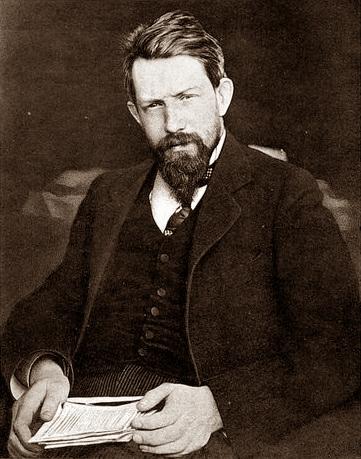
\includegraphics[height=6.2cm,keepaspectratio]{Piotr_Struve}}}{By Неизвестен [Public domain], via Wikimedia Commons}}
\vspace*{-3cm}
\begin{center}
\begin{tikzpicture}[text width=2.7cm, align=flush center,
grow cyclic,
level 1/.style={level distance=3.5cm,sibling angle=90},
level 2/.style={text width=2cm, font=\footnotesize, level distance=3cm,sibling angle=30}]
\node[text width=3.2cm] {\textsc{\myhref{http://ru.wikipedia.org/wiki/\%D0\%A1\%D1\%82\%D1\%80\%D1\%83\%D0\%B2\%D0\%B5\%2C_\%D0\%9F\%D1\%91\%D1\%82\%D1\%80_\%D0\%91\%D0\%B5\%D1\%80\%D0\%BD\%D0\%B3\%D0\%B0\%D1\%80\%D0\%B4\%D0\%BE\%D0\%B2\%D0\%B8\%D1\%87}{\textbf{П.Б. Струве}} (1870-1944)}}
  child[sibling angle=180, level distance=4.6cm] { node[text height=\onelen, text width=9cm, anchor=east] (one) {\usebox{\one}}
  }
  child[level distance=4.6cm] { node[text height=\threelen, text width=9cm,anchor=west] {\usebox{\three}}
  }
  child[sibling angle=-90, level distance=3.5cm, text width=9cm, text height=\twolen, anchor=north] { node {\usebox{\two} }
};
\begin{scope}[every annotation/.style={font=\normalsize, fill=white, text width=9cm}]
\node [annotation, below] at (one.south) {
\textbf{Избранные труды}\medskip
\begin{enumerate}[label={[\arabic*]}]
\item Хозяйство и цена, 1913\,г.
\end{enumerate}
};
\end{scope}
\end{tikzpicture}
\end{center}

\end{document}
